\documentclass[12pt]{article}
\usepackage{tikz}
\usepackage{amssymb}
\usepackage{amsmath}

\begin{document}

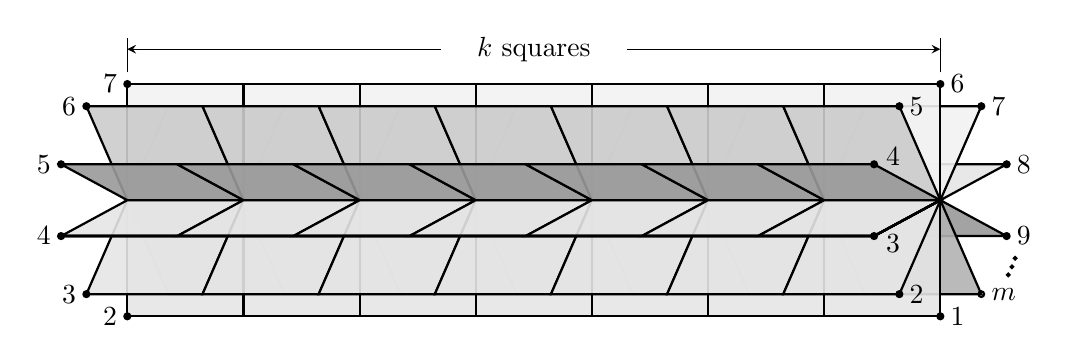
\begin{tikzpicture}[scale=1.475,style=thick]
\def\vr{2.5pt}
\def\sh{7pt}
\def\fac{0.6}

\definecolor{gray0}{rgb}{0.95,0.95,0.95}
\definecolor{gray1}{rgb}{0.9,0.9,0.9}
\definecolor{gray2}{rgb}{0.8,0.8,0.8}
\definecolor{gray3}{rgb}{0.7,0.7,0.7}
\definecolor{gray4}{rgb}{0.6,0.6,0.6}

\def\alpha{18}
\foreach \x in {0,1,2,3,4,5,6} \draw  [fill=gray1, fill opacity=0.9] (\x,0)--({\x+1},0)--({\x+1+\fac*cos(\alpha)},{sin(\alpha)})--({\x+\fac*cos(\alpha)},{sin(\alpha)})--cycle;
\def\alpha{-18}
\foreach \x in {0,1,2,3,4,5,6} \draw [fill=gray4, fill opacity=0.9] (\x,0)--({\x+1},0)--({\x+1+\fac*cos(\alpha)},{sin(\alpha)})--({\x+\fac*cos(\alpha)},{sin(\alpha)})--cycle;

\def\alpha{54}
\foreach \x in {0,1,2,3,4,5,6} \draw  [fill=gray0, fill opacity=0.9] (\x,0)--({\x+1},0)--({\x+1+\fac*cos(\alpha)},{sin(\alpha)})--({\x+\fac*cos(\alpha)},{sin(\alpha)})--cycle;
\def\alpha{-54}
\foreach \x in {0,1,2,3,4,5,6} \draw [fill=gray3, fill opacity=0.9] (\x,0)--({\x+1},0)--({\x+1+\fac*cos(\alpha)},{sin(\alpha)})--({\x+\fac*cos(\alpha)},{sin(\alpha)})--cycle;

\def\alpha{90}
\foreach \x in {0,1,2,3,4,5,6} \draw  [fill=gray0, fill opacity=0.9] (\x,0)--({\x+1},0)--({\x+1+\fac*cos(\alpha)},{sin(\alpha)})--({\x+\fac*cos(\alpha)},{sin(\alpha)})--cycle;
\def\alpha{270}
\foreach \x in {0,1,2,3,4,5,6} \draw [fill=gray1, fill opacity=0.9] (\x,0)--({\x+1},0)--({\x+1+\fac*cos(\alpha)},{sin(\alpha)})--({\x+\fac*cos(\alpha)},{sin(\alpha)})--cycle;
\def\alpha{126}
\foreach \x in {0,1,2,3,4,5,6} \draw  [fill=gray2, fill opacity=0.9] (\x,0)--({\x+1},0)--({\x+1+\fac*cos(\alpha)},{sin(\alpha)})--({\x+\fac*cos(\alpha)},{sin(\alpha)})--cycle;
\def\alpha{234}
\foreach \x in {0,1,2,3,4,5,6} \draw [fill=gray1, fill opacity=0.9] (\x,0)--({\x+1},0)--({\x+1+\fac*cos(\alpha)},{sin(\alpha)})--({\x+\fac*cos(\alpha)},{sin(\alpha)})--cycle;
\def\alpha{162}
\foreach \x in {0,1,2,3,4,5,6} \draw [fill=gray4, fill opacity=0.9] (\x,0)--({\x+1},0)--({\x+1+\fac*cos(\alpha)},{sin(\alpha)})--({\x+\fac*cos(\alpha)},{sin(\alpha)})--cycle;
\def\alpha{198}
\foreach \x in {0,1,2,3,4,5,6} \draw  [fill=gray1, fill opacity=0.9] (\x,0)--({\x+1},0)--({\x+1+\fac*cos(\alpha)},{sin(\alpha)})--({\x+\fac*cos(\alpha)},{sin(\alpha)})--cycle;
\draw (0,0)--(7,0);

\foreach \x in {90,126,162,198,234, 270} \draw ({\fac*cos(\alpha)},{sin(\alpha)})--+(7,0)--(7,0);

\foreach \x in {1,2,3,4,5,6,7,8,9} \draw ({7+\fac*cos(-(\x-9)*36-18)},{sin(-(\x-9)*36-18)}) [fill=black] circle (0.025);
\foreach \x in {1,2,5,6,7,8,9} \draw ({7+\fac*cos(-(\x-9)*36-18)},{sin(-(\x-9)*36-18)}) node [right] {$\x$};
\draw ({7+\fac*cos(158},{sin(158)}) node [right] {$4$};
\draw ({7+\fac*cos(202},{sin(202)}) node [right] {$3$};
\draw ({7+\fac*cos(-54)},{sin(-54)}) circle (0.024)  node [right] {$m$};

\foreach \x in {2,3,4,5,6,7} \draw ({\fac*cos(-(\x-10)*36-18)},{sin(-(\x-10)*36-18)}) [fill=black] circle (0.025) node [left] {$\x$};

\foreach \x in {-30,-35,-40} \draw ({7.125+\fac*cos(\x)},{sin(\x)}) circle (0.01);

\draw [->,>=stealth, thin] (2.7,1.3)--+(-2.7,0);
\draw (3.5,1.3) node {$k$ squares};
\draw [->,>=stealth, thin] (4.3,1.3)--+(2.7,0);
\foreach \x in {0,7} \draw [thin] (\x,1.1)--+(0,0.3);
\end{tikzpicture}

\end{document}